% !TEX root =  master.tex
\chapter{COVID-19 Detection}\label{chapter:detection}


\section{Faster R-CNN}
\sectionauthor{Written by Tobias Richstein}
 
 The Faster R-CNN network architecture proposed in \autocite{ren_faster_2016} by \citeauthor{ren_faster_2016} is an evolutionary step in a line of \acp{R-CNN} which are \acp{CNN} that can perform object detection on images. When given an image, an \ac{R-CNN} is able to predict bounding boxes for detected objects and also classify them. Each predicted bounding box is also given a confidence score that expresses how reliable the model assumes this result is. State of the art Faster \acp{R-CNN} achieve \ac{mAP} scores with an \ac{IoU} threshold of $0.5$ of $0.484$ on a reference COCO object detection validation set making it very well suitable for all kinds of detection tasks such as the one at hand. 
 
 
 Beschreibung Faster RCNN
 
 Beschreibung Resnext
 
 \subsection*{Training of the backbone}
 
 First we trained the ResNeXt network to have a performant backbone that the Faster \ac{R-CNN} can utilize. A reference ResNeXt model architecture and implementation can be obtained directly from the makers of PyTorch \autocite{pytorch_team_resnext_nodate}, which we did. This reference implementation has also been pre-trained on the ImageNet dataset, meaning that we only fine-tune the weights to our use-case. We train the model on the NIH dataset described in section \vref{data:nih} and only expect it to predict the classes of illnesses that can be seen in the X-rays. We encode the ground truths, consisting of the 14 classes of the NIH dataset, as one-hot vectors and therefore also expect output tensors of the same dimension. Like in the original ResNeXt paper, we also use a \acf{SGD} optimizer that has Nesterov acceleration during training. Our learning rate decays over time and follows the equation given below which was originally proposed in \autocite{he_bag_2018} and modified slightly to provide a learning rate floor of $0.05$: 
 
 $$
 \frac{1}{2}\left(1 + \cos\left(\frac{t * \pi}{T}\right)\right) * 0.95 + 0.05
 $$
 
 As described in the ResNeXt paper we load the images and then perform the augmentations necessary to fit the model requirements. To do so, we use a custom dataloader that provides batches of images together with the one-hot encoded ground truth vectors. The augmentation steps done during dataloading include:
 
 \begin{itemize}
 	\item Resize the image to have 256 pixels on the shorter side
 	\item Perform a $224 \times 224$ crop in the center of the resized image
 	\item Normalize the RGB channels to have a mean of $R=0.485; G=0.456; B=0.406$ and a standard deviation of $R=0.229; G=0.224; B=0.225$
 \end{itemize}

To prevent overfitting during training we also randomly apply additional augmentations such as horizontal flips ($p=0.5$), random blurs ($p=0.3$), random rotations of up to 20° ($p=1$) or random erasings of between 1 and 10 percent of the image area ($p=0.3$).

Since we have somewhat limited hardware resources at our disposal in comparison to large scale compute clusters that are often used for such training tasks by researchers, we also apply a method called \textit{Autocasting} to speed up training and allow us to use larger batch sizes. The basis of Autocasting is the ability to use mixed precision during network training. While most frameworks such as PyTorch usually use 32bit floating point numbers (single precision) for all calculations, it has been shown that performing some operations with 16bit representations (half precision) does not penalize accuracy but provides a large speedup since more data can fit in the most often constrained GPU memory and the also constrained data transfer bandwidth can be used more effectively \autocite{micikevicius_mixed_2018}. The GPUs that we have at our disposal also feature special matrix multiplication hardware that works best with half precision numbers, meaning that we profit from mixed precision training in a significant way. The speedup for the ResNeXt training for example was almost twice as fast as before. The decision whether to perform operations at half precision is made automatically by PyTorch when the model is wrapped in an autocasting decorator.

We train the ResNeXt with a batch size of 32 (like in the original paper) and perform 35 epochs. To calculate the loss we use Binary Cross Entropy but with Logits as recommended for mixed precision training which uses the log-sum-exp trick to improve the numerical stability and avoid loss terms that cannot be represented by half precision \autocite{pytorch_team_automatic_nodate}. The loss numbers for the training and validation loss can be seen in \vref{fig:resnet_loss}. It can be seen that in the end some overfit occures where the train loss keeps decreasing and the validation loss stays mostly constant or even increases very slightly. In the end we still decided to use the model after 35 epochs since the loss figures are very good and it also evaluates very well as will be shown later in chapter \vref{chapter:eval_resnext}.

\begin{figure*}
	\centering
	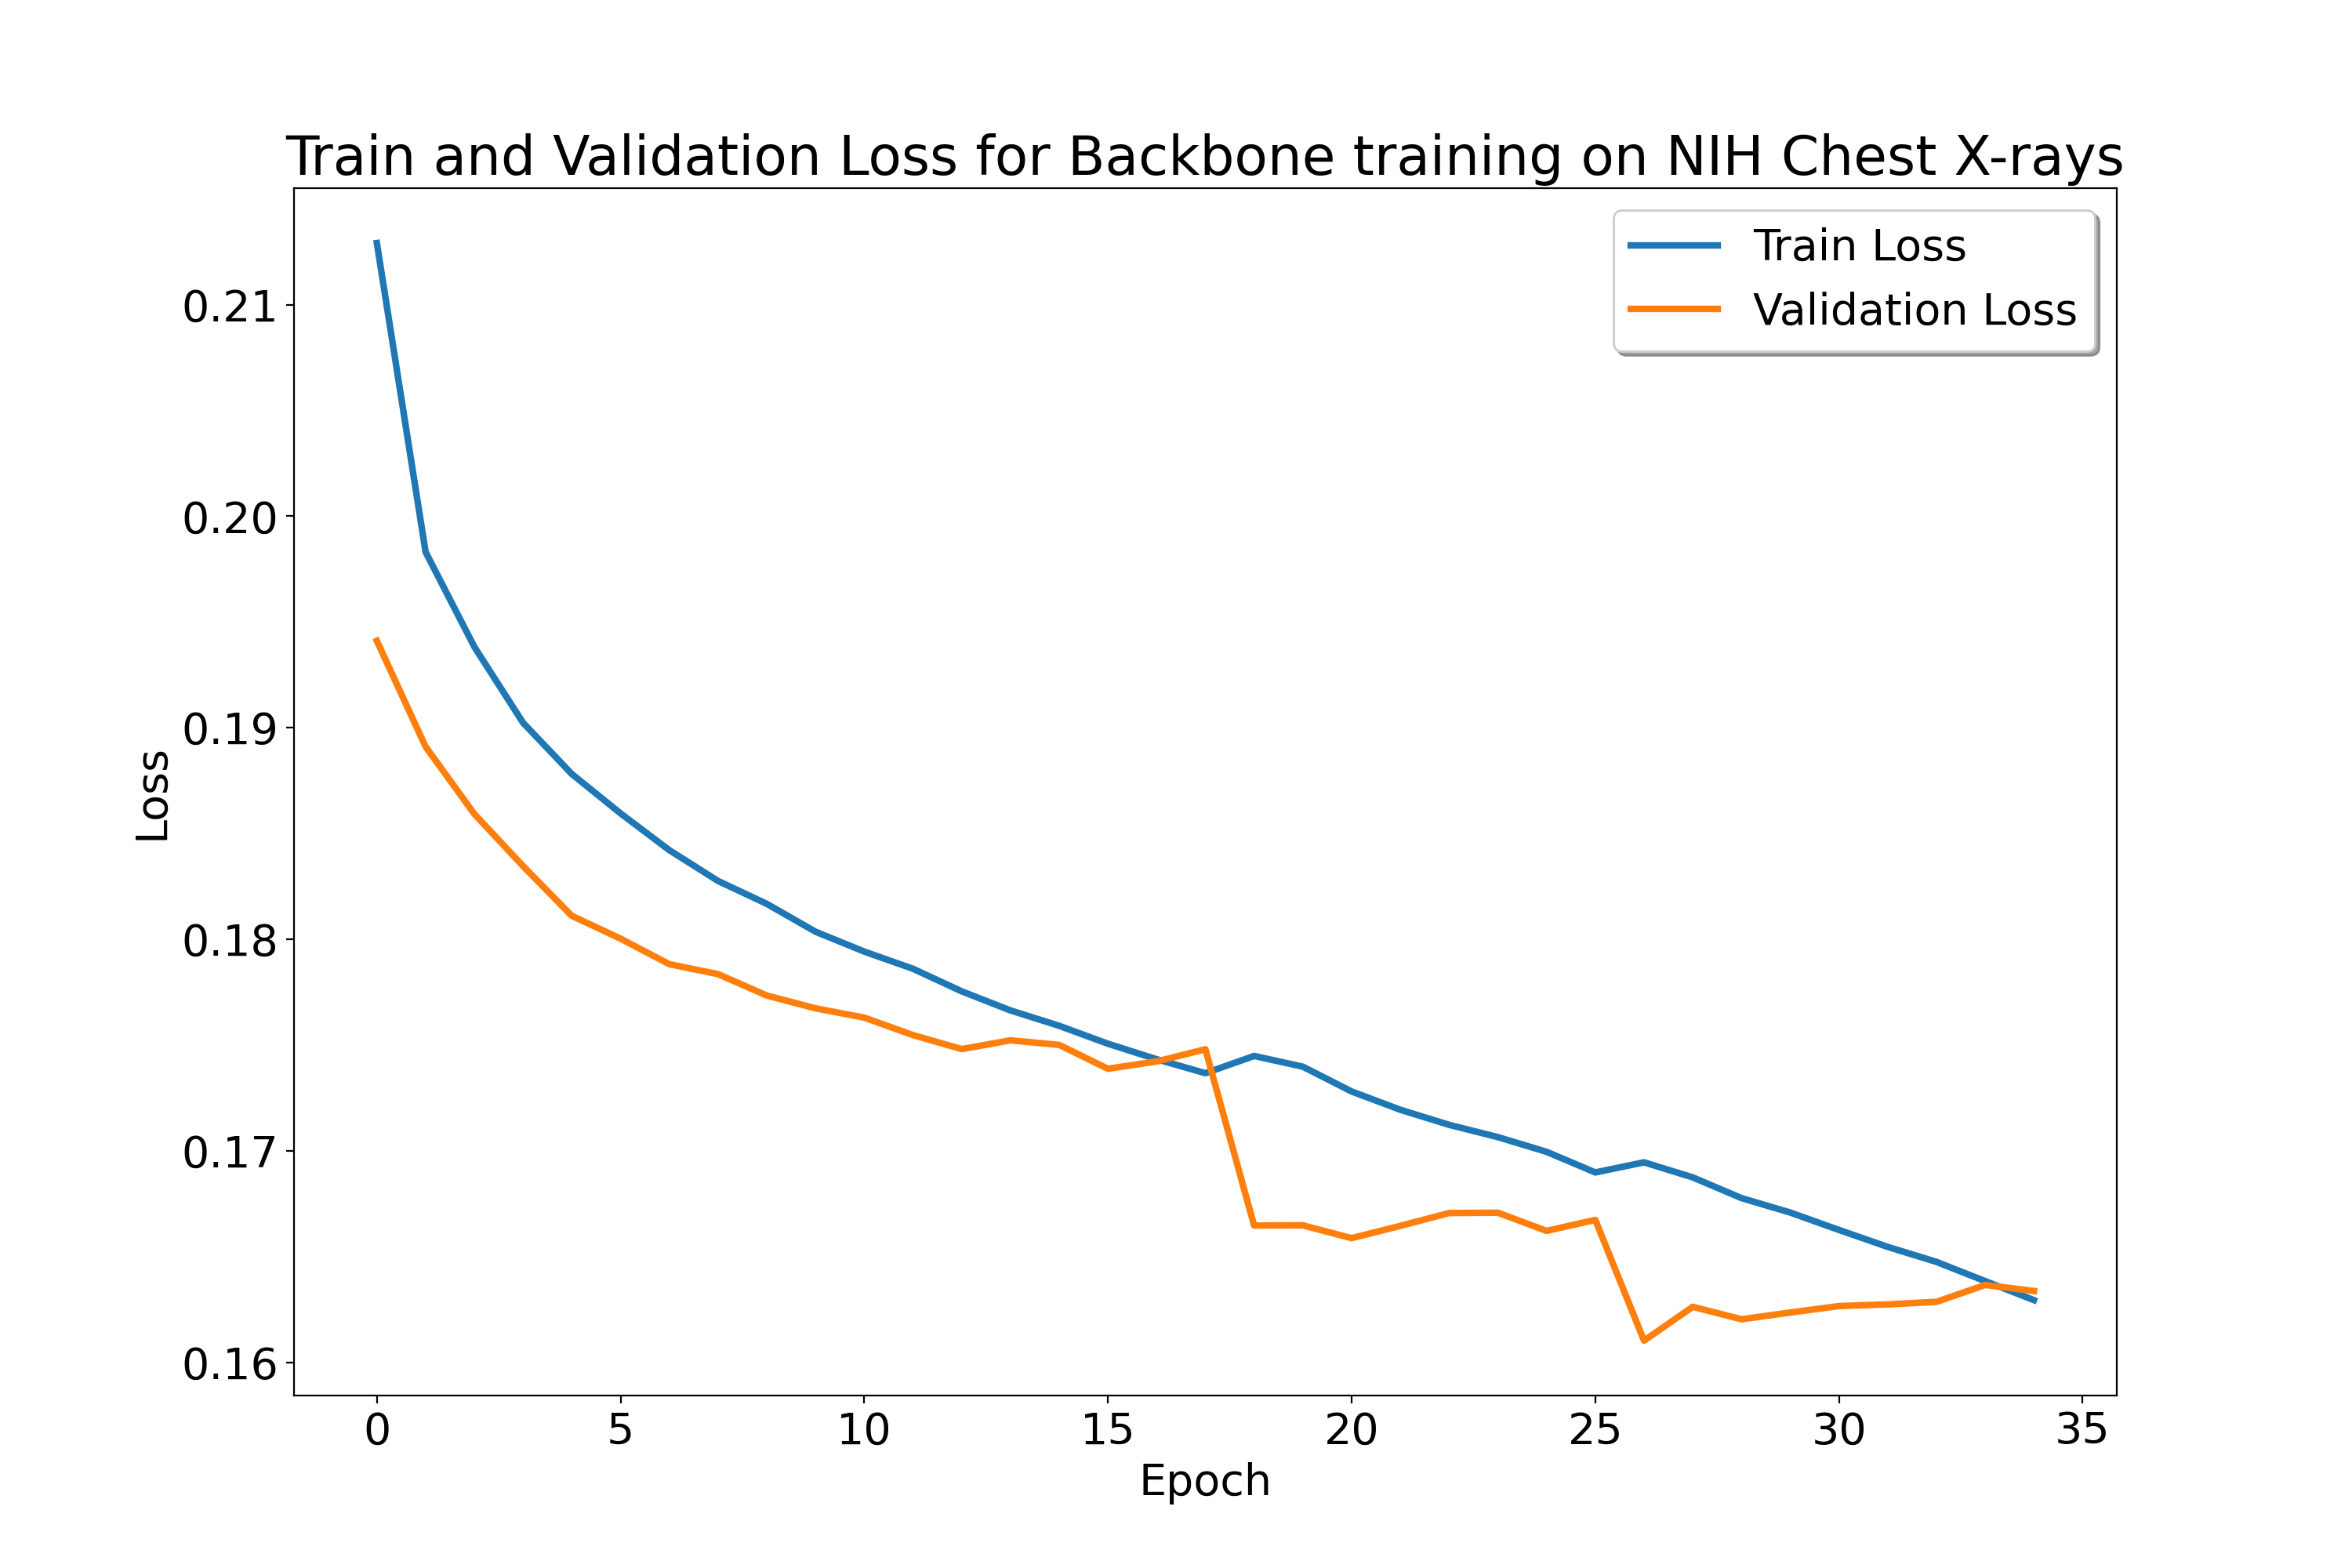
\includegraphics[width=.9\linewidth]{img/loss_backbone_rcnn_35.png}
	\caption{Loss figures of the ResNeXt training}
	\label{fig:resnet_loss}
\end{figure*}

 \subsection*{Training of the Faster R-CNN}

With the backbone network trained, we could now train the Faster R-CNN on the actual detection task of predicting where lung opacities are located in a patient's X-ray image. This training shares a lot of optimizations with the backbone network described above. We use the same \ac{SGD} optimizer and learning rate schedule and train for 50 epochs which does not take too long due to the limited number of training images. We also again use autocasting since the speed improvements are too good to leave out.

Due to the limited number of samples available in the SIIM dataset, we now augment the images more extensively to further prevent overfitting. Because we now have bounding boxes in the aforementioned (?) COCO format we also have to apply all augmentations to those too. To also allow the network to better detect small opacities and details we now train with a much larger image size of $512 \times 512$. We also perform random horizontal flips ($p=0.3$), random shifts with rotations of maximum 20° ($p=0.3$), one of random sharpen ($p=0.5$) or blur ($p=0.25$), random brightness and contrast adjustments ($p=0.3$) and random circular cutouts (max. 6; $p=0.3$). During inference however we pass the inputs as $1024 \times 1024$ images to make the results even clearer. As with the backbone net, we also adjust the RGB channels to fit the required mean and standard deviation values.

Due to the much larger input images and network size we can only train the Faster R-CNN with a batch size of 10 and perform validation with a batch size of 6. During training of a Faster R-CNN multiple loss values have to be taken into account since there are the two tasks of classification and bounding box prediction. Detailed loss figures can be seen in figure \vref{fig:rcnn_loss}. As will be evidenced later in chapter \vref{chapter:eval_rcnn_yolo} after 50 epochs there was already some overfit even though the loss numbers look promising.
 
 \begin{figure*}
 	\centering
 	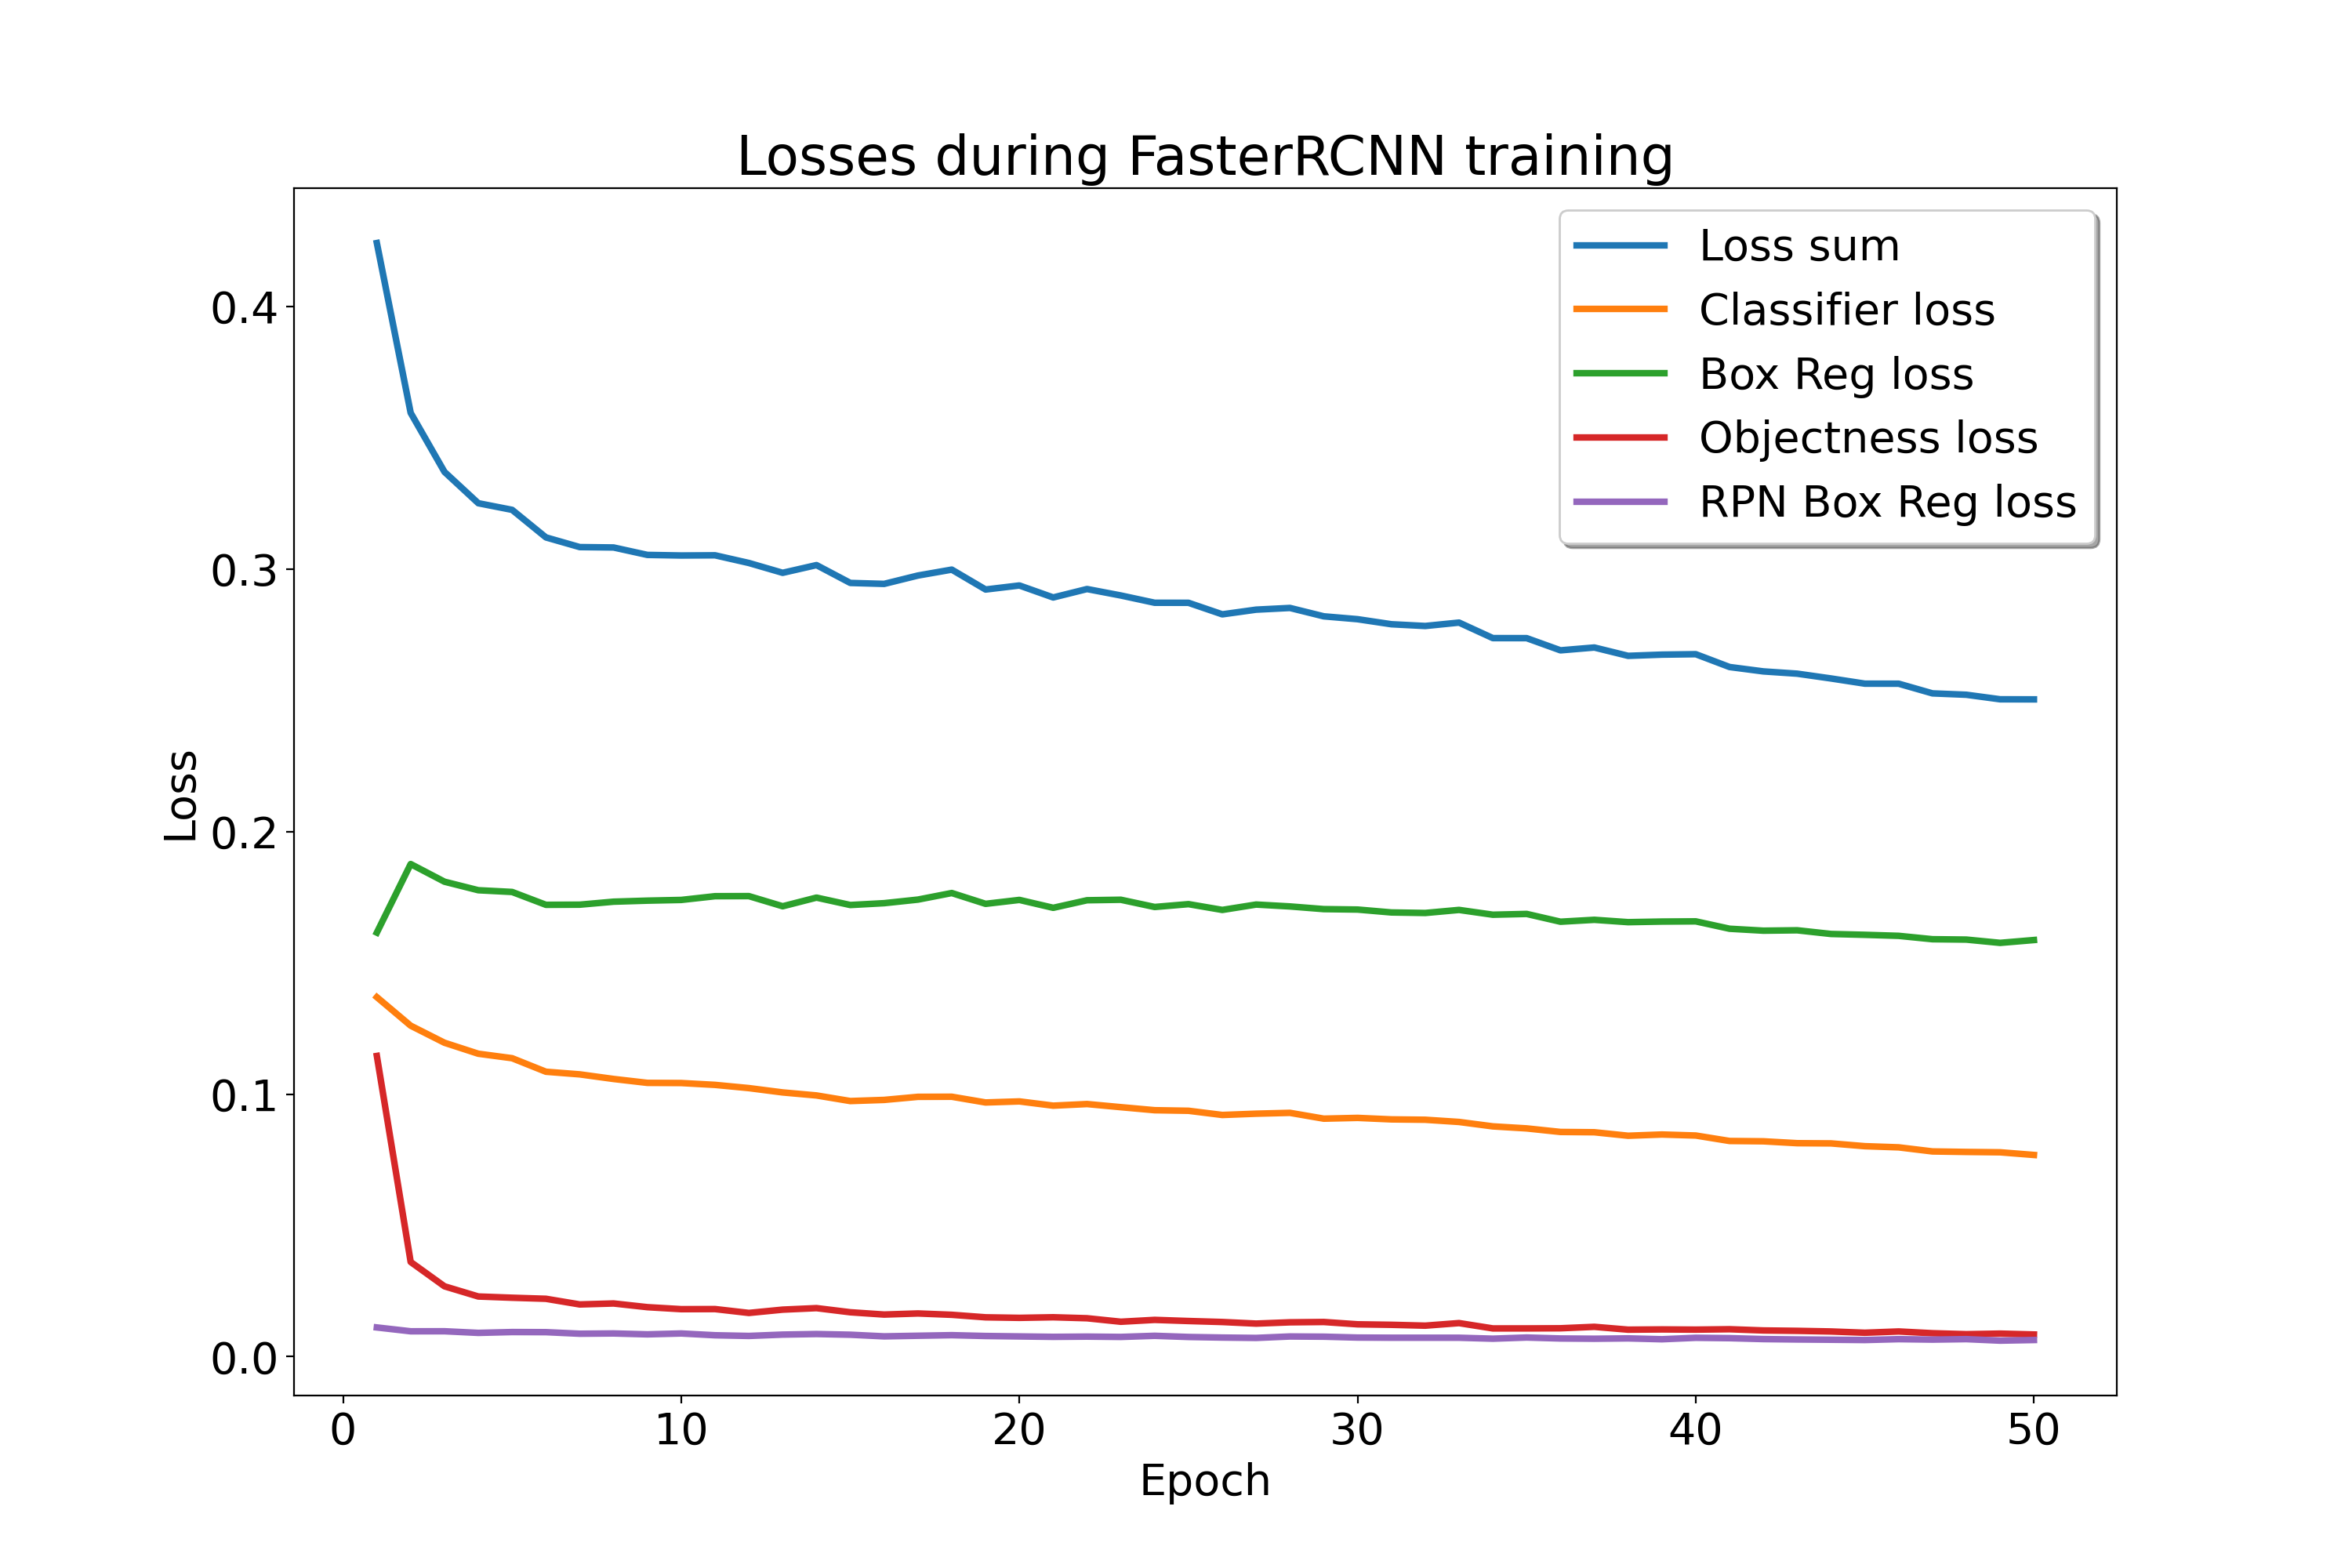
\includegraphics[width=.9\linewidth]{img/loss_fasterrcnn_50.png}
 	\caption{Loss figures of the Faster R-CNN training}
 	\label{fig:rcnn_loss}
 \end{figure*}
 
\section{YOLO}
\sectionauthor{Written by Julian}
 
\section{Study-Level model}
\sectionauthor{Written by Torben}

